\documentclass[11pt,a4paper]{article}
\usepackage[utf8]{inputenc}
\usepackage[T1]{fontenc}
\usepackage{amsmath, amssymb}
\usepackage{amsthm}
\usepackage{booktabs}
\usepackage{pgfplots}
\pgfplotsset{compat=1.18, scaled ticks=false,
  tick label style={/pgf/number format/fixed, /pgf/number format/precision=4, /pgf/number format/1000 sep={}}}
\definecolor{ptblue}{HTML}{1F77B4}
\definecolor{ptred}{HTML}{D62728}
\definecolor{ptgreen}{HTML}{2CA02C}
\definecolor{ptorange}{HTML}{FF7F0E}
\definecolor{ptpurple}{HTML}{9467BD}
\definecolor{ptbrown}{HTML}{8C564B}
\definecolor{ptpink}{HTML}{E377C2}
\definecolor{ptcyan}{HTML}{17BECF}
\definecolor{ptolive}{HTML}{BCBD22}
\definecolor{ptgray}{HTML}{7F7F7F}
\definecolor{ptblack}{HTML}{000000}
\usepackage[margin=2.5cm]{geometry}
\usepackage{hyperref}
\hypersetup{pdftitle={Energy Decay in a Damped Harmonic Oscillator}, pdfauthor={Lena Ortiz}}

\newtheorem{theorem}{Theorem}

\title{Energy Decay in a Damped Harmonic Oscillator}
\author{Lena Ortiz\\ \small Department of Physics, Northfield College}
\date{October 2026}

\begin{document}
\maketitle

\begin{abstract}
We study the free motion of a mass on a linear spring subject to viscous damping. We derive the closed-form solution in the underdamped regime, show that the mechanical energy decays monotonically, and compare the analytic solution with two simple numerical schemes.
\end{abstract}

\section{Introduction}\label{sec:intro}

The damped harmonic oscillator is the simplest model of a system that loses energy to its surroundings~\cite{ref1}. Its equation of motion is
\begin{equation}
  m\ddot{x}+c\dot{x}+kx=0,
\end{equation}
where $m>0$ is the mass, $c\geq0$ the damping coefficient and $k>0$ the spring constant. Dividing by $m$ and writing $\omega_{0}=\sqrt{\frac{k}{}}$ and $\gamma=\frac{c}{(2m)}$ gives the \emph{standard form}.
\begin{equation}
  \ddot{x}+2\gamma\dot{x}+\omega_{0}^{2}x=0.
\end{equation}

\section{Solution}

Substituting $x=e^{\lambda t}$ into REF2 gives the characteristic equation $\lambda^{2}+2\gamma\lambda+\omega_{0}^{2}=0$, whose roots are
\begin{equation}
  \lambda_{\pm}=-\gamma\pm\sqrt{\gamma^{2}-\omega_{0}^{2}.}
\end{equation}
The behaviour depends on the sign of the discriminant:
\begin{equation*}
  \text{regime}=\begin{cases}
\text{underdamped,} & \gamma<\omega_{0}, \\
\text{critically damped,} & \gamma=\omega_{0},
\end{cases}
\end{equation*}
In the underdamped case let $\omega_{d}=\sqrt{\omega_{0}^{2}-\gamma^{2}}$. With $x(0)=x_{0}$ and $\dot{x}(0)=0$ the solution is
\begin{equation}
  x(t)=x_{0}e^{-\gamma t}\left( \cos\omega_{d}t+\frac{\gamma}{\omega_{d}}\sin\omega_{d}t \right).
\end{equation}
Equivalently, with $\boldsymbol{y}=(x,\dot{x})^{T}$, equation REF2 becomes the first-order system
\begin{equation}
  \dot{\boldsymbol{y}}=\begin{pmatrix}
0 & 1 \\
-\omega_{0}^{2} & -2\gamma.
\end{pmatrix}\boldsymbol{y}.
\end{equation}

\begin{theorem}
  The energy $E(t)=\frac{1}{2}m\dot{x}^{2}+\frac{1}{2}kx^{2}$ never increases. More precisely, $\frac{dE}{dt}=-c\dot{x}^{2}\leq0$.
\end{theorem}

\begin{proof}
  Differentiate $E$ and use REF1:
\end{proof}

\begin{align*}
  \frac{dE}{dt} &=m\dot{x}\ddot{x}+kx\dot{x} \\
   &=\dot{x}(m\ddot{x}+kx)=-c\dot{x}^{2}.
\end{align*}

\section{Numerical check}

We integrated REF2 with $\omega_{0}=2$, $\gamma=0.2$ and $x_{0}=1$ on $tin[0,10]$, using the explicit Euler method and the classical fourth-order Runge--Kutta method (RK4)~\cite{ref2}. For each step size $h$ we:

\begin{enumerate}
  \item integrated from $t=0$ to $t=10$ with $\frac{10}{h}$ steps;
  \item compared every step with the exact solution REF4;
  \item recorded the largest absolute difference.
\end{enumerate}

Table~\ref{tab:errors} lists the results and REFF shows the exact solution.

\begin{table}[htbp]
  \centering
  \caption{Maximum absolute error on $[0,10]$.}
  \label{tab:errors}
  \begin{tabular}{lcc}
    \toprule
    \textbf{Step $h$} & \textbf{Euler} & \textbf{RK4} \\
    \midrule
    0.100 & 8.51 $\times10^{-1}$ & 5.00 $\times10^{-5}$ \\
    0.050 & 2.50 $\times10^{-1}$ & 3.10 $\times10^{-6}$ \\
    0.025 & 1.06 $\times10^{-1}$ & 1.93 $\times10^{-7}$ \\
    \bottomrule
  \end{tabular}
\end{table}

\begin{figure}[htbp]
  \centering
  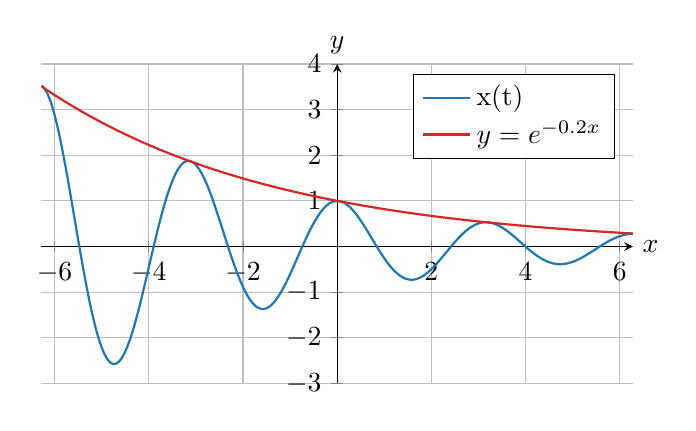
\begin{tikzpicture}
    \begin{axis}[
      width=0.75\linewidth,
      height=0.465\linewidth,
      axis lines=middle,
      xmin=-6.28, xmax=6.28,
      ymin=-3, ymax=4,
      xtick distance=2,
      ytick distance=1,
      grid=major,
      xlabel={$x$},
      ylabel={$y$},
      xlabel style={at={(ticklabel* cs:1)}, anchor=west},
      ylabel style={at={(ticklabel* cs:1)}, anchor=south},
      unbounded coords=jump,
      restrict y to domain=-10:11,
      legend pos=north east,
      legend cell align=left
    ]
      \addplot[ptblue, thick, domain=-6.28:6.28, samples=200] {e^(-0.2*x)*(cos(deg(1.99*x)) + 0.1005*sin(deg(1.99*x)))};
      \addlegendentry{x(t)}
      \addplot[ptred, thick, domain=-6.28:6.28, samples=200] {e^(-0.2*x)};
      \addlegendentry{$y = e^{-0.2x}$}
    \end{axis}
  \end{tikzpicture}
  \caption{The solution REF4 for $\gamma=0.2$, $\omega_{0}=2$ and its envelope $\pm e^{-\gamma t}$.}
\end{figure}

Two things stand out:

\begin{itemize}
  \item Euler's error is large because the method \textbf{adds} energy at every step, which works against the physical damping.
  \item Halving $h$ divides the RK4 error by about $16=2^{4}$, as expected for a fourth-order method.
\end{itemize}

\begin{thebibliography}{9}
\bibitem{ref1} H. Goldstein, C. Poole and J. Safko, \emph{Classical Mechanics}, 3rd ed., Addison-Wesley, 2002.
\bibitem{ref2} E. Hairer, S. P. Nørsett and G. Wanner, \emph{Solving Ordinary Differential Equations I}, 2nd ed., Springer, 1993.
\end{thebibliography}

\end{document}
